\section{Forces on a 2-dimensional body}
\begin{framed}
Ideal potential flows:
\begin{equation}
\vec{\nabla}\cdot\vec{u}=0=\vec{\nabla}\times\vec{u}\Rightarrow\vec{\nabla}\cdot\vec{\nabla}\phi = \left(\ppdiff{}{x}+\ppdiff{}{y}\right)\phi=0
\end{equation}
Where is the Euler equation? Do we need it?
\end{framed}
For an ideal potential flow the Euler equation
\begin{equation}
\rho \left(\pdiff{\vec{u}}{t}+\left(\vec{u}\cdot\vec{\nabla}\right)\vec{u}\right) = \rho \vec{f} - \vec{\nabla}p + \mu\left(\vec{\nabla}\cdot\vec{\nabla}\right)\vec{u}
\end{equation}
reduces to the Bernoulli equation:
\begin{equation}
\vec{\nabla}\left(\frac{\rho}{2}\vec{u}^2+p\right)=0.
\end{equation}
With the Bernoulli equation (leftover from the Euler equation) we can calculate the force on the "obstacle" (\fref{fig:2dim-body}) from the surrounding flow:
\begin{align}
\vec{F} &= \int_{S(u)}(-p(\vec{r}))d\vec{A} = -\int_{S(u)}\left(p_0-\frac{\rho}{2}\vec{u}^2(\vec{r})\right)d\vec{A} \\
&= \frac{\rho}{2}\int_{S(u)}\vec{u}^2(\vec{r})d\vec{A}\\
&= L\vec{e}_y +\underbrace{D\vec{e}_x}_{=0}.
\end{align}
$\vec{L}$ is the lift force and $\vec{D}$ is the drag force. The last term equals zero because there is no friction.

\begin{figure}[!h]
    \centering
    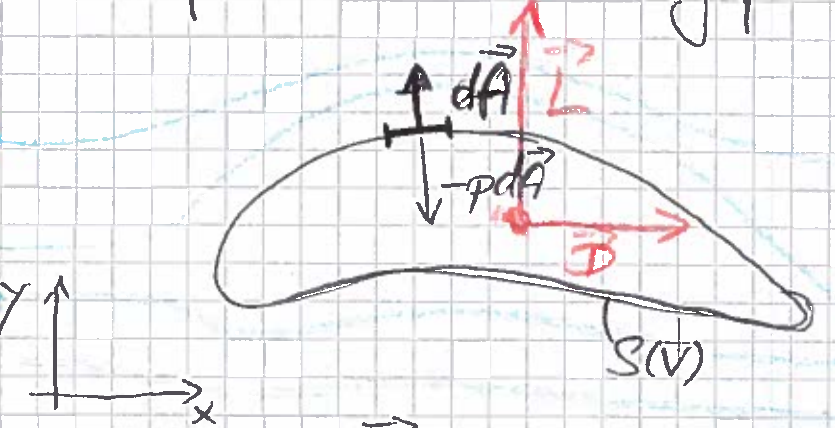
\includegraphics[width=.5\textwidth]{week4/2dim-body}\\
    \caption{}
    \label{fig:2dim-body}
\end{figure}

\begin{figure}[!h]
    \centering
    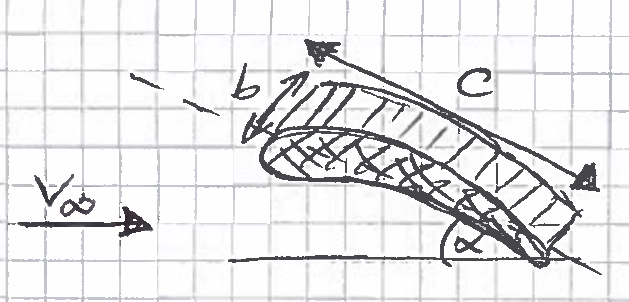
\includegraphics[width=.4\textwidth]{week4/generic-lift2}\\
    \caption{}
    \label{fig:generic-lift2}
\end{figure}

Lift coefficient
\begin{equation}
C_L = \frac{L}{\frac{\rho}{2}v_\infty^2 b c}
\end{equation}
Drag coefficient (for the case that friction is non-zero):
\begin{equation}
C_D = \frac{D}{\frac{\rho}{2}v_\infty^2 b c}
\end{equation}

\begin{figure}[!h]
    \centering
    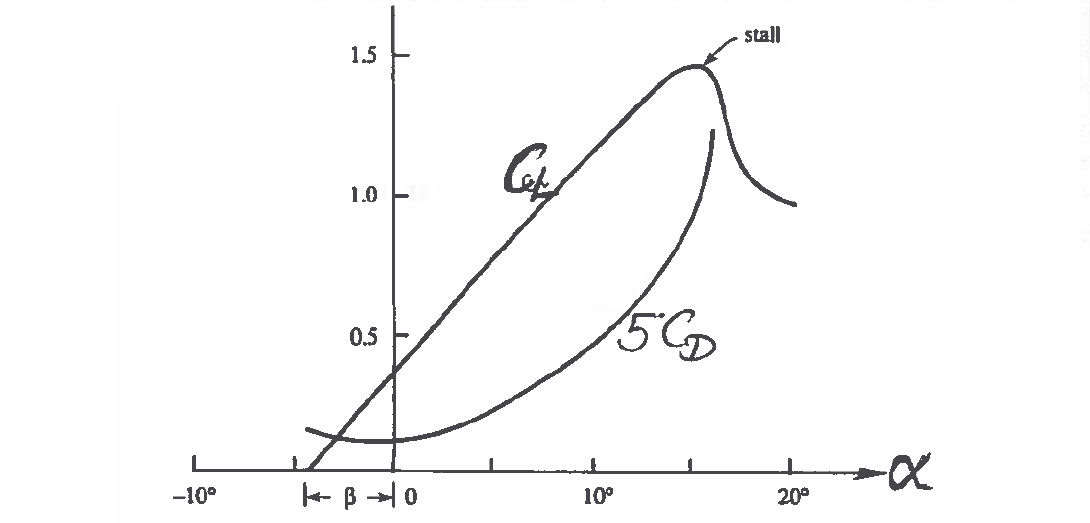
\includegraphics[width=.5\textwidth]{week4/generic-lift}\\
    \caption{Generic lift and drag coefficients vs. angle of attack. There is lift at $\alpha=0$ so the foil shape has nonzero camber. The drag increase is almost quadratic with increasing angle of attack.}
    \label{fig:generic-lift}
\end{figure}


\subsection{Turbine blade}
The lift force pulls the rotor blade of a wind turbine forward. See \fref{fig:turbine-blade}.
\begin{figure}[!h]
    \centering
    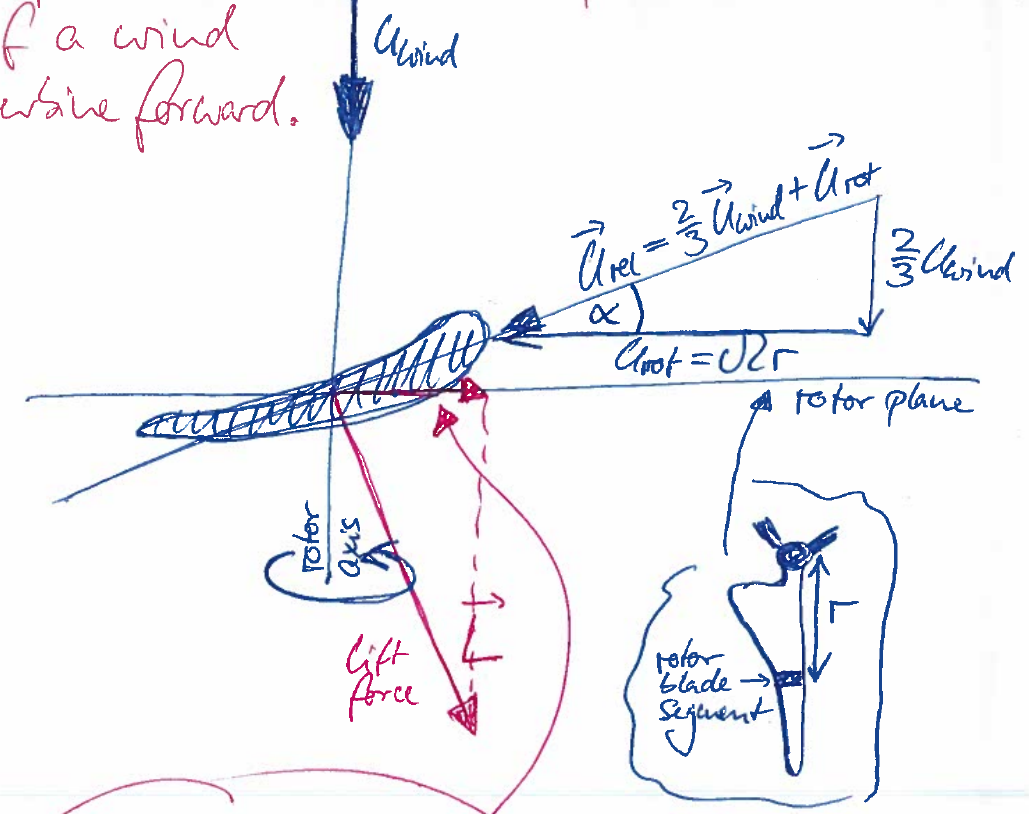
\includegraphics[width=.6\textwidth]{week4/turbine-blade}\\
    \caption{}
    \label{fig:turbine-blade}
\end{figure}


\subsection[Sailing against the wind]{Sailing against the wind (KCD 14.9)}
People have sailed without the aid of an engine for thousands of years and have known
how to reach an upwind destination. Actually, it is not possible to sail exactly against the
wind, but it is possible to sail at $\approx$ 40-45$^\circ$ to the wind. \fref{fig:sailing-wind} shows
how this is made possible by the aerodynamic lift on the sail, which is a piece of stretched and stiffened
cloth. The wind speed is U, and the sailing speed is V, so that the apparent wind speed relative
to the boat is $U_r$. If the sail is properly oriented, this gives rise to a lift force perpendicular
to U$_\text{r}$ and a drag force parallel to U$_\text{r}$. The resultant force F can be resolved into a driving
component (thrust) along the motion of the boat and a lateral component. The driving
component performs work in moving the boat; most of this work goes into overcoming
the frictional drag and in generating the gravity waves that radiate outward from the hull.
The lateral component does not cause much sideways drift because of the shape of the
hull. It is clear that the thrust decreases as the angle $\theta$ decreases and normally vanishes
when $\theta$ is $\approx$ 40-45$^\circ$ . The energy for sailing comes from the wind field, which loses kinetic
energy after passing the sail.

\begin{figure}[!h]
    \centering
    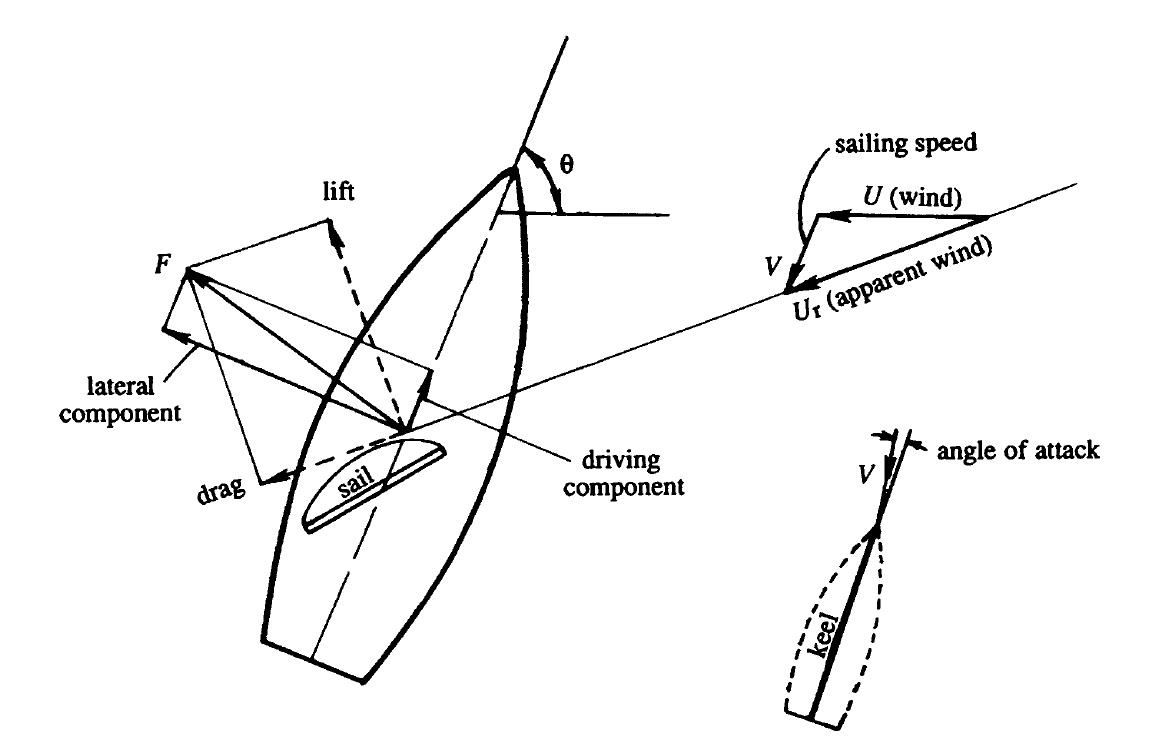
\includegraphics[width=.6\textwidth]{week4/sailing-wind}\\
    \caption{Principle of sailing against the wind. A small component of the sail’s lift pushes the boat forward at an angle $\theta$ < 90$^\circ$ to the wind. Thus by traversing a zig-zag course at angles $\pm\theta$, a sailboat can reach an upwind destination. A sailboat’s keel may make a contribution to its upwind progress too.}
    \label{fig:sailing-wind}
\end{figure}

\newpage
\subsection{Reynolds number}
Fluid around a cylinder can create several real flow patterns. See \fref{fig:reynolds-cylinder}.

\begin{figure}[p]
    \centering
    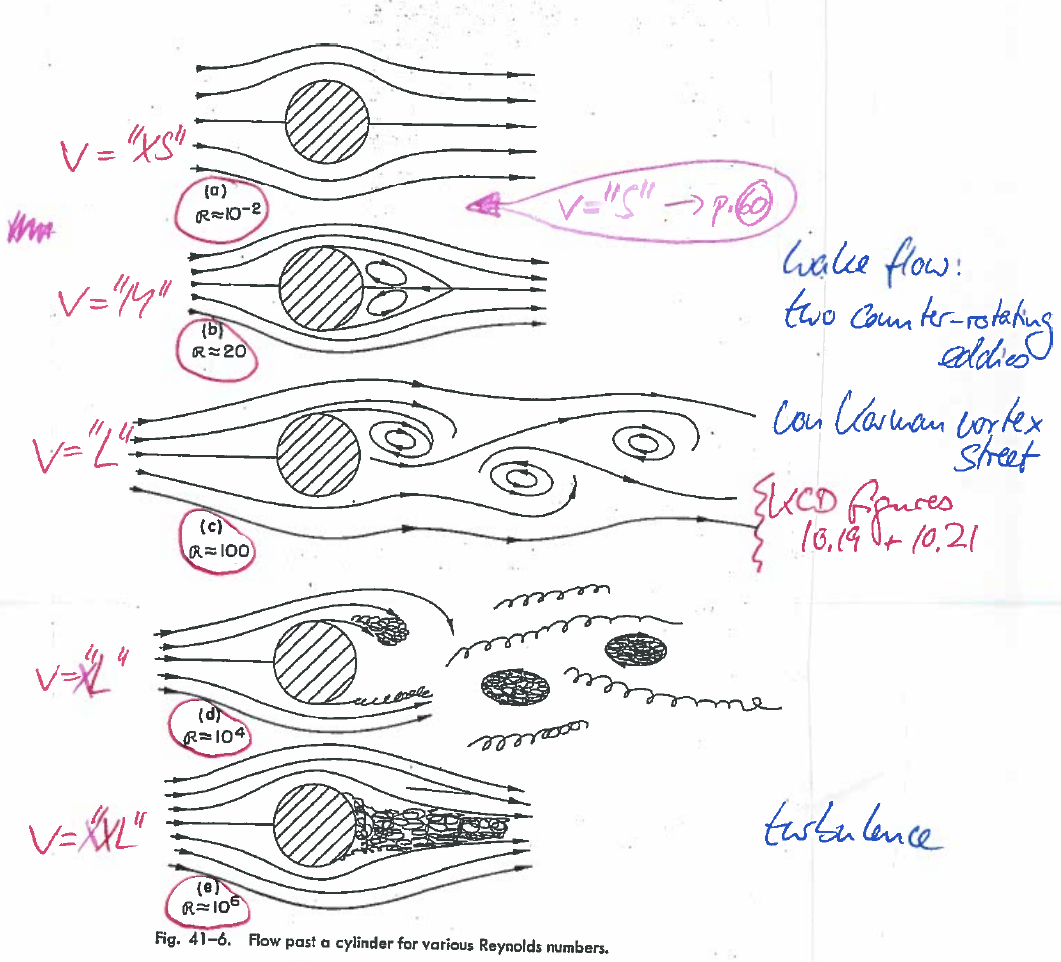
\includegraphics[width=\textwidth]{week4/reynolds-cylinder}\\
    \caption{}
    \label{fig:reynolds-cylinder}
\end{figure}

\textbf{Questions:}
\begin{enumerate}
\item Why so many different flows?
\item What causes and characterizes them?
\end{enumerate}
Certainly friction, i.e. viscosity, will have something to do with it.

\begin{align}
0 &= \rho_0 \left[\pdiff{\vec{u}}{t}+\left(\vec{u}\cdot\vec{\nabla}\right)\vec{u}\right] + \vec{\nabla}p - \mu \left(\vec{\nabla}\cdot\vec{\nabla}\right) \vec{u} \\
&= \rho_0\left[\frac{U}{T}\pdiff{\vec{u}'}{t'}+\frac{U^2}{L}\left(\vec{u}'\cdot\vec{\nabla}'\right)\vec{u}'\right] + \frac{\rho_0 U^2}{L}\vec{\nabla}'p'-\mu\frac{U}{L^2}\left(\vec{\nabla}\cdot\vec{\nabla}\right)'\vec{u}' \\
&= \rho_0\frac{U^2}{L} \left\lbrace \pdiff{\vec{u}'}{t'}+\left(\vec{u}'\cdot\vec{\nabla}'\right)\vec{u}'+\vec{\nabla}'p'-\frac{\mu}{\rho_0 LV} \left(\vec{\nabla}\cdot\vec{\nabla}\right)'\vec{u}' \right\rbrace
\end{align}
where $L$ is the characteristic length, $U$ is the characteristic velocity, $T=L/U$ is the characteristic time, and $P=\rho_0U^2$ the characteristic pressure.

Reynolds number:
\begin{equation}
Re = \frac{\rho_0 L U}{\mu}
\end{equation}

\begin{framed}
\textbf{Remark:} law of similarity

If two flows have the same geometry (object) and the same Reynolds number, but a different absolute scale it means that the two flows are similar (identical, except for a scale transformation). Applications of this is wind tunnel experiments of air wings, wind turbine blades, cars, etc.
\end{framed}

The Reynolds number
\begin{equation}
Re = \frac{\rho_0 L U}{\mu} = \frac{\rho_0 U^2/L}{\mu U/L},
\end{equation}
is the inertia force density divided by the friction force density.

\begin{figure}[p]
    \centering
    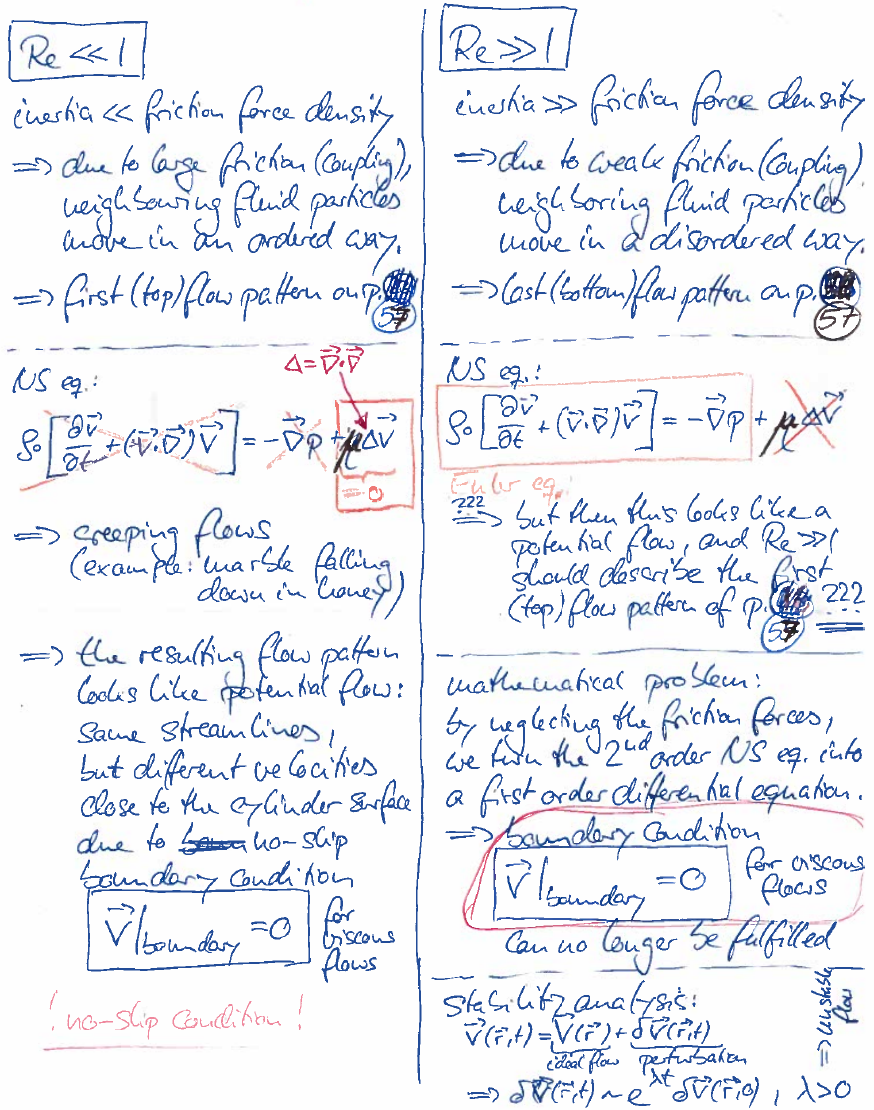
\includegraphics[width=\textwidth]{week4/reynolds-numbers}\\
    \caption{This should be presented in text in a better way.}
    \label{fig:reynolds-numbers}
\end{figure}

\begin{figure}[p]
    \centering
    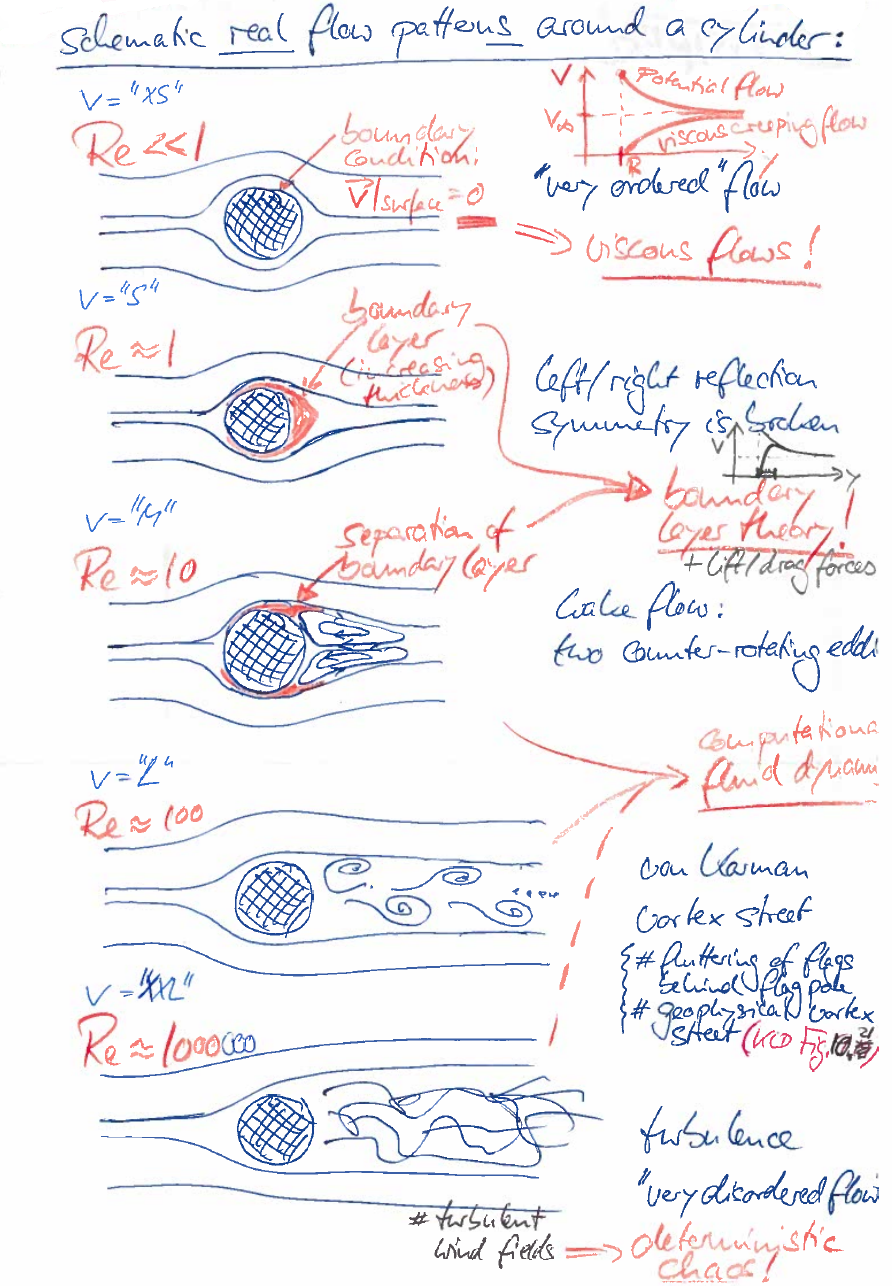
\includegraphics[width=\textwidth]{week4/schematic-flows}\\
    \caption{}
    \label{fig:schematic-flows}
\end{figure}


\newpage
\subsection{Viscous pipe flow}

\begin{figure}[ht]
    \centering
    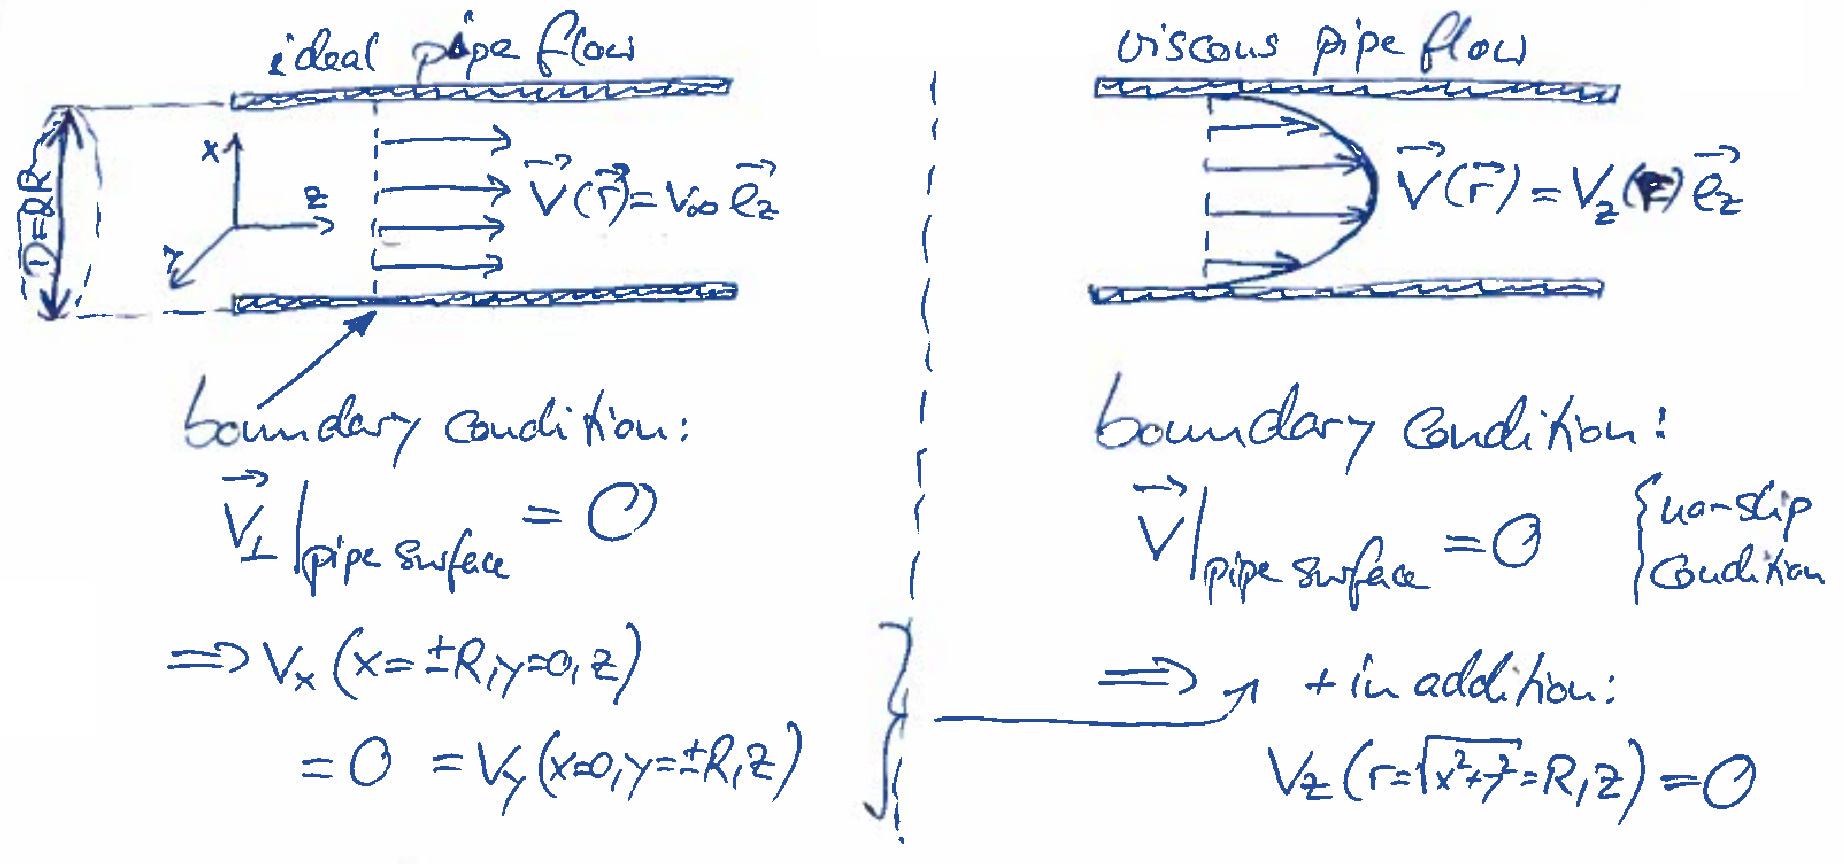
\includegraphics[width=\textwidth]{week4/viscous-pipe-flow}\\
    \caption{}
    \label{fig:viscous-pipe-flow}
\end{figure}

Task: calculate velocity profile $u_z=u_z(r)$ for the viscous pipe flow.

Navier-Stokes equation
\begin{equation}
\rho_0\underbrace{\pdiff{\vec{u}}{t}}_{=0}+\rho_0\underbrace{\left(\vec{u}\cdot\vec{\nabla}\right)}_{=0}\vec{u} = \underbrace{\vec{f}_\mathrm{ext}}_{=0}-\vec{\nabla}p+\mu\left(\vec{\nabla}\cdot\vec{\nabla}\right)\vec{u}
\end{equation}
The second term on the left-hand side vanishes because of the incompressibility condition
\begin{equation}
0=\vec{\nabla}\cdot\vec{u}=\partial_xu_x+\partial_yu_y+\partial_zu_z = \partial_zu_z
\end{equation}
with $u_x=u_y=0$ and
\begin{equation}
\left(\vec{u}\cdot\vec{\nabla}\right)\vec{u} = u_z\partial_z
\begin{pmatrix}
0\\0\\u_z
\end{pmatrix} = 0.
\end{equation}
\begin{align}
\vec{\nabla}p = \mu\left(\ppdiff{}{x}+\ppdiff{}{y}\right)u_z\vec{e}_z\\
\leadsto
\left(\vec{\nabla}p\right)_x &= \left(\vec{\nabla}p\right)_y = 0 \\
\leadsto
p &= p(z)
\end{align}

\begin{align}
\mu\left(\vec{\nabla}\cdot\vec{\nabla}\right) v_z(r) &= \frac{\mu}{r}\pdiff{}{r}\left(r\pdiff{u_z(r)}{r}\right) \\
&= \pdiff{p(z)}{z} \require \mathrm{constant}
\end{align}

\begin{align}
\pdiff{p(z)}{t}&=c \\
\leadsto
p(z) &= cz+d \\
&= \frac{p(z=L)-p(z=0)}{L}z+p(z=0)\\
&= -\frac{\Delta p}{L}z + p(z=0)
\end{align}

\begin{align}
\frac{\mu}{r}\pdiff{}{r}\left(r\pdiff{v_z(r)}{r}\right) &= c = -\frac{\Delta p}{L} \\
\leadsto
r\pdiff{v_z(r)}{r} &= -\frac{\Delta p}{\mu L}\frac{r^2}{2} + D_1 \\
\leadsto
v_z(r) &= -\frac{\Delta p}{4\mu L}r^2 + D_1 \ln r + D_ 2 \\
\leadsto
v_z(r) &= \frac{\Delta p}{4\mu L}\left( R^2 - r^2\right)
\end{align}

Fluid mass per time passing through pipe cross-section:
\begin{equation}
\diff{M}{t} = \int_0^R\rho_0 v_z(r)2\pi r dr = \frac{\pi\rho_0 R^4\Delta p}{8\mu L}
\end{equation}
This is the Hagen-Poiseuille law.
\begin{framed}
\textbf{Remark:} this law allows to determine the viscosity:
\begin{equation}
\left\lbrace \underbrace{\rho_0,R,L}_\mathrm{known} \quad,\quad \underbrace{\Delta p,\diff{M}{t}}_\mathrm{measured} \right\rbrace \Rightarrow \mu
\end{equation}
\end{framed}

\begin{framed}
\textbf{Remark:} "Ohm's Law"

\begin{align}
\Delta p = \Delta u \ &,\quad \diff{M}{t} = I\\
\leadsto
I &= \frac{\pi\rho_0 R^4}{8L\mu}
\end{align}

{\center
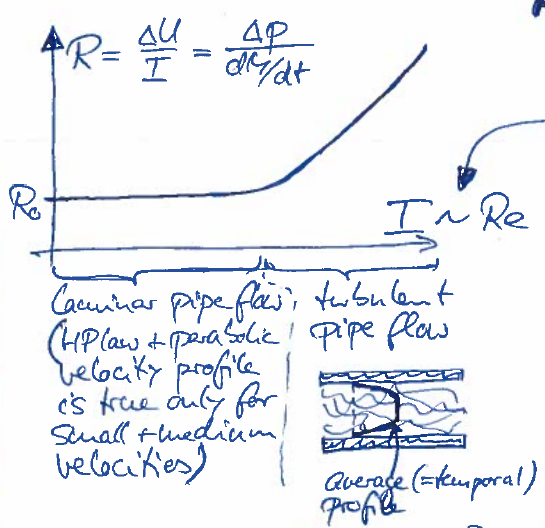
\includegraphics[width=.4\textwidth]{week4/ohms-law}\\
}

\begin{equation}
R = R_0\cdot f(Re)
\end{equation}
with
\begin{equation}
f(Re\rightarrow0)=1
\end{equation}
we conclude that turbulence increases pipe resistance. This is important for the operation of oil and gas pipelines.
\end{framed}




\newpage
\subsection{Boundary layers}

\begin{figure}[ht]
    \centering
    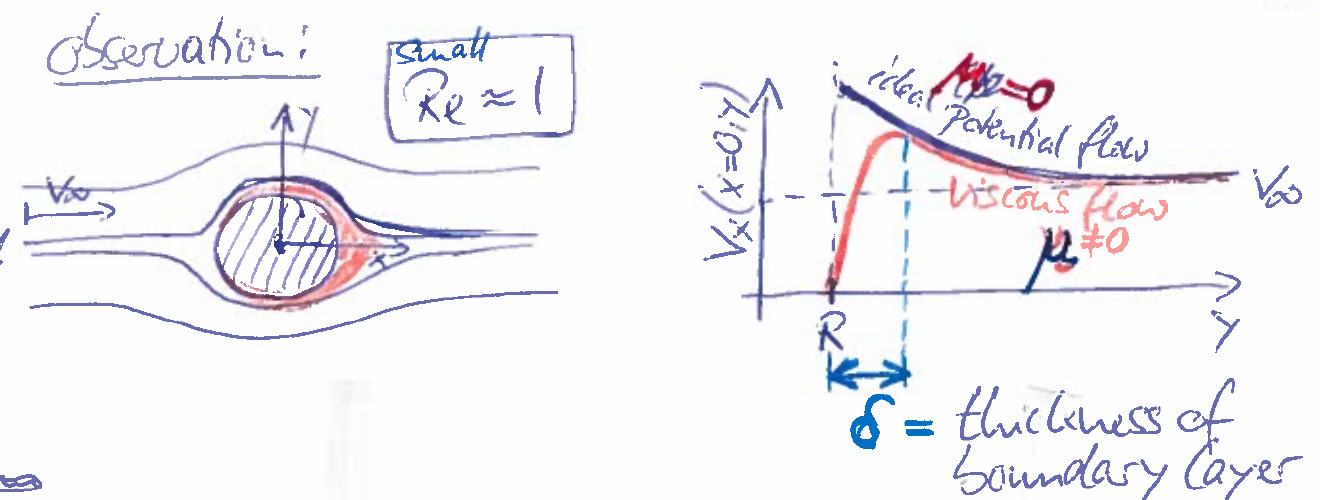
\includegraphics[width=\textwidth]{week4/boundary-layers}\\
    \caption{}
    \label{fig:boundary-layers}
\end{figure}

Idea of boundary layer theory:
\begin{enumerate}
\item within the boundary layer the velocity increases from zero to the ideal flow velocity
\item inside the boundary layer we use the Navier-Stokes equation (with friction)
\item outside the boundary layer we use the Euler equation without friction i.e. ideal potential flow
\item at the boundary surface we match the inside solution with the outside solution
\end{enumerate}

Derivation of the (laminar) boundary layer equations. Approximation to the Navier-Stokes equation inside the boundary layer. See \fref{fig:laminar-boundary}.

\begin{figure}[ht]
    \centering
    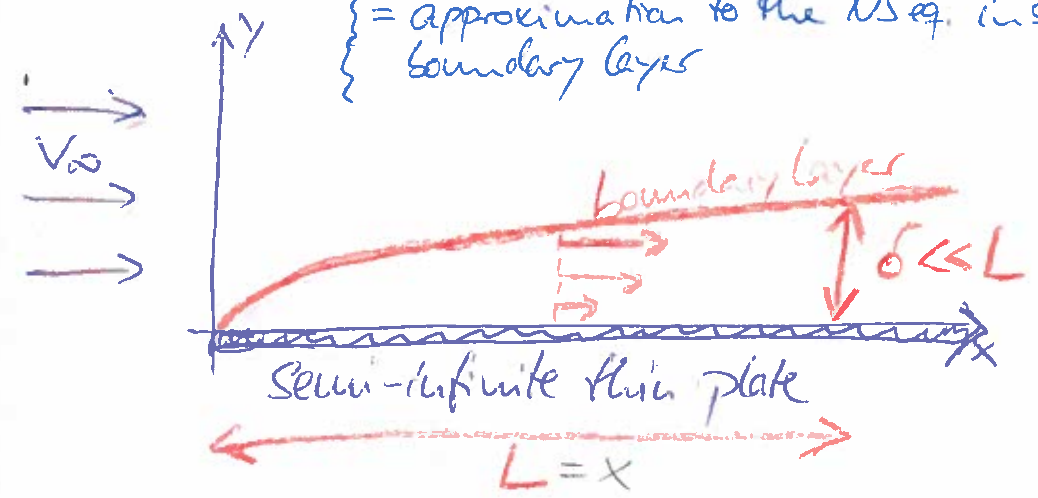
\includegraphics[width=.7\textwidth]{week4/laminar-boundary}\\
    \caption{}
    \label{fig:laminar-boundary}
\end{figure}

In the following we determine $\delta = \delta(x)$ (\fref{fig:laminar-boundary}) without solving the Navier-Stokes equation.

Incompressible flow:
\begin{align}
\vec{\nabla}\cdot\vec{u} &= \pdiff{v_x}{x} + \pdiff{v_y}{y} = 0 \\
&= \mathcal{O} \left(\frac{v_\infty}{L}\right) + \mathcal{O} \left(\frac{v_y}{\delta}\right) \\
\leadsto
\mathcal{O}(v_y) &= \delta\frac{v_\infty}{L} = \frac{\delta}{L}v_\infty
\end{align}

Navier-Stokes equation (x-component):
\begin{equation}
v_x\pdiff{v_x}{x} + v_y\pdiff{v_x}{y} = -\frac{1}{\rho_0}\pdiff{p}{x} + \frac{\mu}{\rho_0}\ppdiff{v_x}{x} + \frac{\mu}{\rho_0}\ppdiff{v_x}{y}
\end{equation}
\begin{equation}
\mathcal{O} \left(\frac{v_\infty^2}{L}\right) \require \mathcal{O} \left(\frac{\mu}{\rho_0}\frac{v_\infty}{\delta^2}\right)
\end{equation}

\begin{equation}
\left(\frac{\delta}{L}\right)^2 \sim \frac{\mu}{\rho_0 L v_\infty} = \frac{1}{Re}
\end{equation}
The larger the Reynolds number, the thinner the boundary layer. This holds for $Re \leq \SI{1e5}{}-\SI{1e6}{}$, above that the boundary layer becomes turbulent, and is no longer laminar.

\begin{equation}
\delta(x) \sim \sqrt{\frac{\mu x}{\rho_0 v_\infty}}
\end{equation}


Navier-Stokes equation (y-component):
\begin{equation}
v_x\pdiff{v_y}{x} + v_y\pdiff{v_y}{y} = -\frac{1}{\rho_0}\pdiff{p}{y} + \frac{\mu}{\rho_0}\ppdiff{v_y}{x} + \frac{\mu}{\rho_0}\ppdiff{v_y}{y}
\end{equation}

\begin{equation}
\pdiff{p}{y} = 0 \Rightarrow p = p(x)
\end{equation}


\textbf{Prandtl equations:} laminar boundary layer equations
\begin{align}
v_x\pdiff{v_x}{x}+v_y\pdiff{v_x}{y} &= -\frac{1}{\rho_0}\pdiff{p(x)}{x}+\frac{\mu}{\rho_0}\ppdiff{v_x}{y} \\
\pdiff{v_x}{x}+\pdiff{v_y}{y}&=0
\end{align}

\textbf{Example:} Solution of Prandtl equations for laminar boundary flow around semi-infinite plate

\begin{equation}
p=p(x) \Rightarrow p(x)|_\mathrm{inside} = p(x)|_\mathrm{outside}
\end{equation}

Outside boundary layer:
\begin{align}
v_x|_\mathrm{outside} &= v_x = v_\infty = \mathrm{constant} \\
v_y|_\mathrm{outside} &= 0
\end{align}

Bernoulli equation:
\begin{align}
p(x) + \frac{\rho_0}{2}v_x^2 &= \mathrm{constant}\\
\leadsto
p(x) &= \mathrm{constant} \\
\leadsto
\pdiff{p(x)}{x} &= 0
\end{align}

Similarity ansatz:
\begin{equation}
v_x(x,y) = v_\infty g\left(\frac{y}{\delta(x)}\right)
\end{equation}
Except for a rescaling with $\delta(x)$ the velocity $v_x(x,y)$ looks like the same for all $x$.
\begin{figure}[ht]
    \centering
    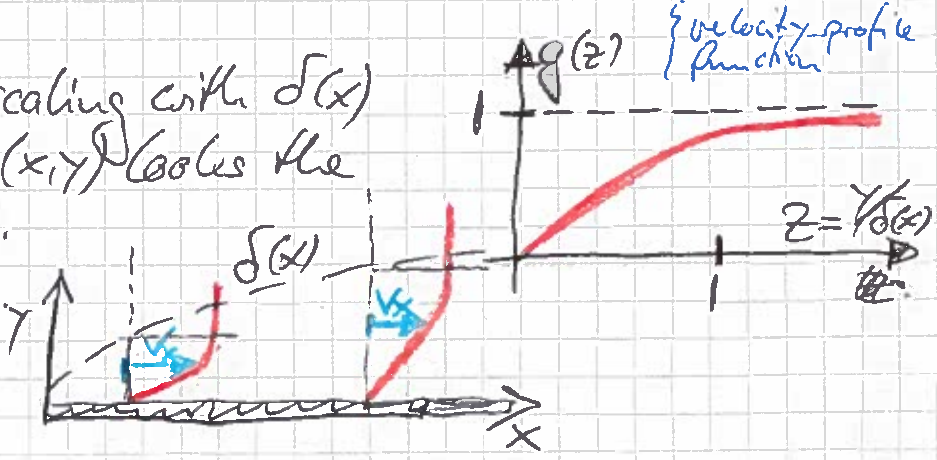
\includegraphics[width=.7\textwidth]{week4/boundary-ansatz}\\
    \caption{}
    \label{fig:boundary-ansatz}
\end{figure}


\noindent\makebox[\linewidth]{\rule{\textwidth}{0.5pt}}

\textbf{Question:} does the similarity ansatz work?

\begin{align}
\pdiff{v_x}{x}+\pdiff{v_y}{y} &= 0 \\
\leadsto
v_x = \pdiff{\psi}{y} \ &, \quad v_y = -\pdiff{\psi}{x}
\end{align}

\begin{equation}
\psi(x,y) = v_\infty\delta(x)f\left(\frac{y}{\delta(x)}\right)
\end{equation}

\begin{align}
v_x=\pdiff{\psi}{y} &= v_\infty\delta(x)\diff{f(z}{z}\diff{z}{y} \\
&= v_\infty \delta(x) \diff{f(z)}{z}\frac{1}{\delta(x)}\\
&= v_\infty \diff{f(z)}{z} \\
&\require v_\infty g(z)
\end{align}

\begin{equation}
f' = \diff{f(z)}{z}g(z)
\end{equation}

\noindent\makebox[\linewidth]{\rule{\textwidth}{0.5pt}}

\begin{align}
v_y &= -\pdiff{\psi}{x} \\
&=  -v_\infty\diff{\delta(x)}{x}f(z) - v_\infty \delta(x)\diff{f(z)}{z}\diff{z}{x}\\
&= v_\infty \left[-f + \frac{y f'}{\delta}\right] \diff{\delta(x)}{x}
\end{align}

\begin{align}
\pdiff{v_x}{x} &= \left(v_\infty f''\right)\left(\frac{-y}{\delta^2}\right)\diff{\delta(x)}{x} = -\frac{v_\infty y f''}{\delta^2}\diff{\delta(x)}{x} \\
\pdiff{v_x}{y} &= (v_\infty f'') \frac{1}{\delta} = \frac{v_\infty f''}{\delta} \\
\pdiff{v_x}{y} &= \frac{v_\infty f''}{\delta^2}
\end{align}

\begin{align}
\begin{split}
v_x\pdiff{v_x}{x} + v_y\pdiff{v_x}{y} - \frac{\mu}{\rho_0}\ppdiff{v_x}{y} &=
-(v_\infty f') \left(\frac{v_\infty y f''}{\delta^2} \diff{\delta(x)}{x}\right) \\
&\hspace{5mm} + \left(v_\infty\left[-f\frac{yf'}{\delta}\right]\diff{\delta(x)}{x}\right) \left(\frac{v_\infty f''}{\delta}\right) \\
&\hspace{5mm} -\frac{\mu}{\rho_0} \left(\frac{v_\infty f''}{\delta^2}\right)
\end{split} \\
&= -\frac{v_\infty^2}{\delta}\diff{\delta}{x} ff'' - \frac{\mu}{\rho_0} \frac{v_\infty}{\delta^2}f'''\\
&= 0
\end{align}

\begin{equation}
\frac{\rho_0 v_\infty}{\mu} \delta(x) \diff{\delta(x)}{x} = -\frac{f'''(z)}{f(z)f''(z)} \require c_1^2
\end{equation}

\begin{equation}
\delta\diff{\delta}{x} = \frac{1}{2}\diff{\delta^2}{x} = c_1^2\frac{\mu}{\rho_0v_\infty}\\
\end{equation}

\begin{equation}
\delta^2 = 2c_1^2 \frac{\mu}{\rho_0v_\infty}x + c_2
\end{equation}
$c_2=0$ since $\delta(x=0)=0$.

\begin{equation}
\delta(x) = c_1\sqrt{\frac{2\mu}{\rho_0v_\infty}x}
\end{equation}

\begin{equation}
\delta(x)=\sqrt{\frac{\mu}{\rho_0v_\infty}x}
\end{equation}
$c_1=\frac{1}{\sqrt{2}}$. Freedom of choice because of arbitrary definition of $\delta$; for example, $v_x(y=\delta)=0.99v_\infty$ or $v_x(x=\delta)=0.95v_\infty$.

This is the same result as the order of magnitude calculation when we calculated the x-component of the Navier-stokes equation earlier in this section.

\begin{equation}
f'''(z) +\frac{1}{2} f(z)f''(z) = 0
\end{equation}

\begin{equation}
f(z)\ddiff{f(z)}{z}+2\dddiff{f(z)}{z}=0
\end{equation}
This is Blasius' equation. A special case of the more general Falker-Skan equation.


\subsection{Separation of boundary layers (64-65)}

Boundary condition at the wall:
\begin{equation}
v_x(x,y=0) = v_y(x,y=0)=0
\end{equation}

Prandtl equation (with pressure)
\begin{equation}
v_x\pdiff{v_x}{x}+v_y\pdiff{v_x}{y} = -\frac{1}{\rho_0}\pdiff{p}{x}+\frac{\mu}{\rho_0}\ppdiff{v_x}{y}
\end{equation}
If we are very close to the wall, the two terms on the left side equal zero. We then have
\begin{equation}
\pdiff{p(x,y=0)}{x}=\mu\ppdiff{v_x(x,y=0)}{y}
\end{equation}

\begin{figure}[!h]
    \centering
    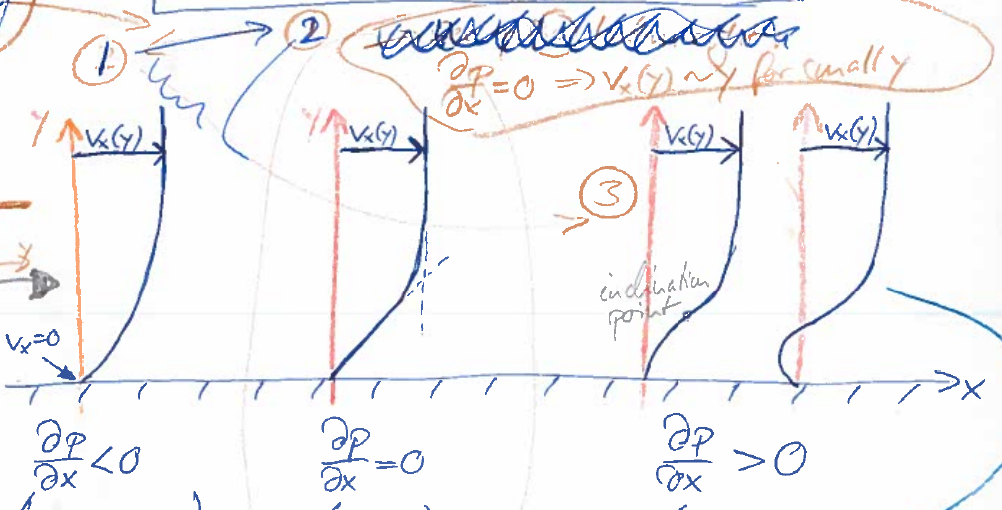
\includegraphics[width=.9\textwidth]{week5/wall-boundary}\\
    \caption{}
    \label{fig:wall-boundary}
\end{figure}

\begin{figure}[!h]
    \centering
    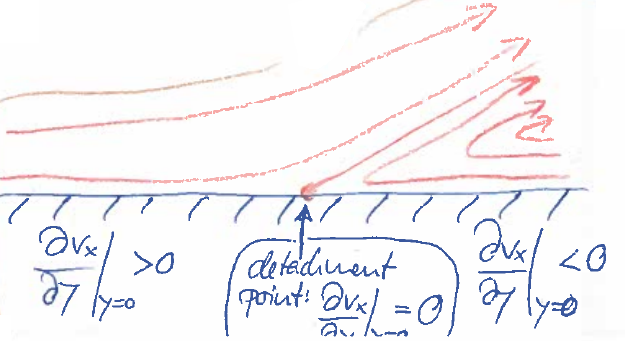
\includegraphics[width=.5\textwidth]{week5/detachment-point}\\
    \caption{}
    \label{fig:detachment-point}
\end{figure}

\newpage
\textbf{Example:} flow around cylinder

\begin{figure}[!h]
    \centering
    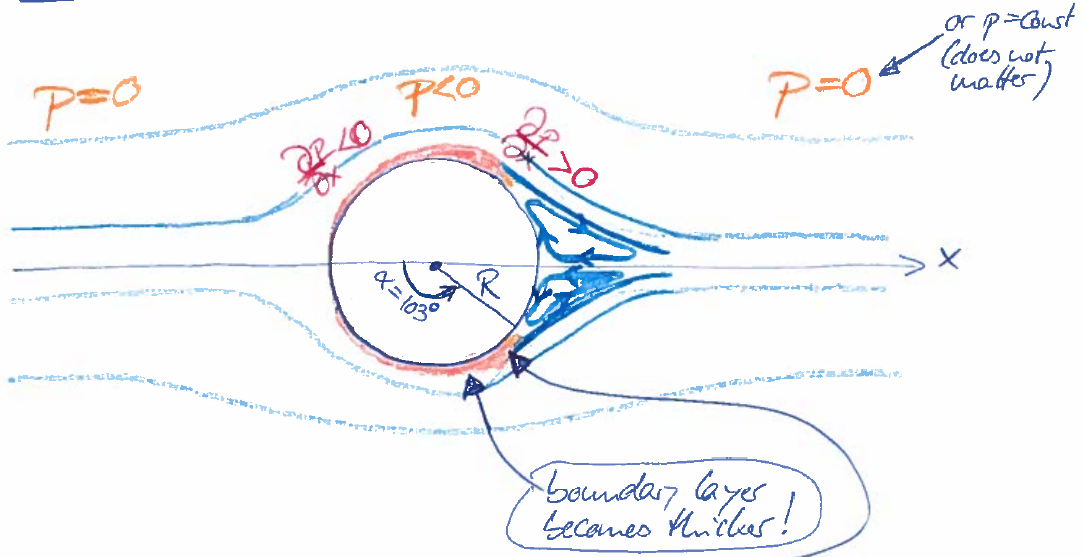
\includegraphics[width=.8\textwidth]{week5/cylinder-flow}\\
    \caption{}
    \label{fig:cylinder-flow}
\end{figure}

The detachment point is at the separation of the boundary layer. When $v\approx0$ there is no kinetic energy to run against the pressure gradient.

\begin{framed}
\textbf{Remark:} separation of boudnary layers is a big issue in mechanical engineering; for example: design of airfoils, wind-turbine blades etc.
{\center
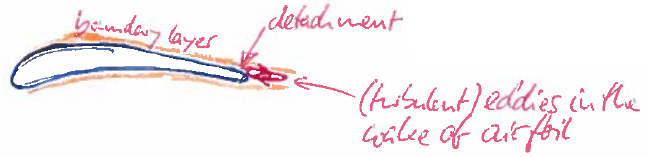
\includegraphics[width=.4\textwidth]{week5/detachment-eddies}\\
}
In case of separation the lift decreases, which can lead to airplane crash. It would also lead to a substantial rise in the overall drag (more friction). This would require more engine power and therefore more fuel for an airplane. For a wind turbine it would means less power generation.

Engineer's dream: construct airfoils without turbulent wake to mimic shark skin or fish scales.
\end{framed}

\subsection{Solution of Prandtl equations for free boundary layers (66-71)}

\fref{fig:2d-laminar-jet} shows a 2-dimensional laminar jet flow generated from a flow through a long slit streaming into a resting fluid.

\begin{figure}[!h]
    \centering
    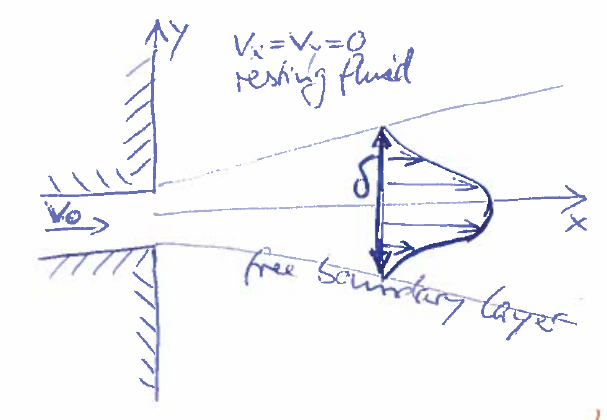
\includegraphics[width=.6\textwidth]{week5/2d-laminar-jet}\\
    \caption{}
    \label{fig:2d-laminar-jet}
\end{figure}

We use the Prandtl equations with the similarity ansatz:
\begin{equation}
v_x(x,y)=v_\mathrm{max}(x)g\left(\frac{y}{\delta(x)}\right)
\end{equation}

\begin{equation}
\pdiff{v_x}{x}+\pdiff{v_y}{y}=0 \Rightarrow v_x=\pdiff{\psi}{y},\quad v_y=-\pdiff{\psi}{x}
\end{equation}

\begin{equation}
\psi = v_\mathrm{max}(x)\delta(x)f\left(\frac{y}{\delta(x)}\right)
\end{equation}

\begin{equation}
\pdiff{\psi}{y}=v_\mathrm{max}\delta f'\frac{1}{\delta}=v_\mathrm{max}f'=v_\mathrm{max}g=v_x
\end{equation}

\begin{equation}
v_y=-\pdiff{\psi}{x}=-v'_\mathrm{max}\delta f-v_\mathrm{max}\delta'f-v_\mathrm{max}\delta f'\frac{(-y)\delta'}{\delta^2}
\end{equation}

\begin{align}
\partial_xv_x &= v'_\mathrm{max}f'+v_\mathrm{max}f''\frac{(-y)\delta'}{\delta^2} \\
\partial_yv_x &= v_\mathrm{max} f''\frac{1}{\delta}\\
\partial^2_xv_x &= \frac{v_\mathrm{max}}{\delta^2}f'''
\end{align}

\begin{align}
\begin{split}
v_x\partial_x v_x+v_y\partial_yv_x-\frac{\mu}{\rho_0}\partial^2_yv_x &= v_\mathrm{max}f'\left\lbrace v'_\mathrm{max}f' - v_\mathrm{max}\frac{y\delta'}{\delta^2}f''\right\rbrace \\
&\hspace{5mm}-\left\lbrace v'_\mathrm{max}\delta f + v_\mathrm{max}d'f-v_\mathrm{max}\frac{y\delta'}{\delta}f'\right\rbrace v_\mathrm{max}\frac{1}{\delta}f'' \\
&\hspace{5mm}-\frac{\mu}{\rho_0^2} \frac{v_\mathrm{max}}{\delta^2}f'''
\end{split}\\
\begin{split}
&= v_\mathrm{max}v'_\mathrm{max}f'^2-v_\mathrm{max}v'_\mathrm{max}ff''-v_\mathrm{max}^2\frac{\delta'}{\delta}ff'' \\
&\hspace{5mm}-\frac{\mu}{\rho_0}\frac{v_\mathrm{max}}{\delta^2}f'''\label{eq:free-boundary}
\end{split} \\
&\require0
\end{align}
All four terms in \eqref{eq:free-boundary} have the form $\alpha_i(x)\beta_i(x)$ for $(i=1,...,4)$. The sum of these four terms has to be zero. This means that $\alpha_1(x)\sim\alpha_2(x)\sim\alpha_3(x)\sim\alpha_4(x)$.

Ansatz:
\begin{align}
v_\mathrm{max}(x) &= c_1x^m\\
\delta(x) &= c_2 x^n
\end{align}

\begin{framed}
\textbf{Remark:} we expect $m<0$ (decreasing velocity with penetration depth) and $n>0$ (increasing thickness of jet with penetration depth).
\end{framed}

Sum of the 4 terms:
\begin{equation}
c_1^2mx^{2m-1}(f'^2-ff'')-c_1^2x^{2m}\frac{n}{x}ff'' - \frac{\mu}{\rho_0}\frac{c_1}{c_2^2}\frac{x^m}{x^{2n}}f'''=0
\end{equation}

\begin{equation}
2m-1 = m-2n
\end{equation}

\begin{equation}
m(f'^2-ff'')nff''-\frac{\mu}{\rho_0}\frac{1}{c_1c_2^2}f'''=0
\end{equation}
This differential equation determines the velocity profile
\begin{equation}
g\left(\frac{y}{\delta(x)}\right)=f'\left(\frac{y}{\delta(x)}\right)
\end{equation}
of the jet. We are not going to solve this, but we want to know $m$ and $n$, because they determine $v_\mathrm{max}(x)$ and $\delta(x)$. We need a second equation for $m$ and $n$.

\textbf{Second equation:} conservation of momentum flux.
Momentum flux through the red plane in \fref{fig:momentum-flux} is identical to the momentum flux through the blue plane. This means that the integrated momentum flux does not depend on $x$.
\begin{figure}[!h]
    \centering
    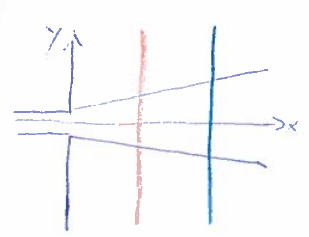
\includegraphics[width=.4\textwidth]{week5/momentum-flux}\\
    \caption{}
    \label{fig:momentum-flux}
\end{figure}

\begin{align}
\mathrm{momentum} & =\rho_0\Delta V\cdot v_x\\
&= \rho_0\Delta Av_x\Delta tv_x
\end{align}

Momentum flux:
\begin{equation}
\frac{\mathrm{momentum}}{\Delta A \Delta t} = \rho_0 v_x^2
\end{equation}

\noindent\makebox[\linewidth]{\rule{\textwidth}{0.5pt}}
\textbf{Proof of conservation of momentum flux}

If
\begin{equation}
\int_{-\infty}^\infty \rho_0v_x^2(x)dy=\mathrm{constant}
\end{equation}
then
\begin{equation}
\diff{}{x}\int_{-\infty}^\infty \rho_0v_x^2(x)dy=0
\end{equation}

\begin{align}
\diff{}{x}\int_{-\infty}^\infty \rho_0v_x^2(x)dy &= 2\rho_0\int_
{-\infty}^\infty\left(v_x\pdiff{v_x}{x}\right)dy \\
&= 2\mu\pdiff{v_x}{y}\biggm\vert_{-\infty}^\infty-2\rho_0\int_{-\infty}^\infty v_y\pdiff{v_x}{y}dy \\
&=-2\rho_0v_xv_y\biggm\vert_{-\infty}^\infty + 2\rho_0 \int_{-\infty}^\infty\pdiff{v_y}{y}dy \\
&= -2\rho_0\int_{-\infty}^\infty v_x\pdiff{v_x}{x}dy\\
&= 0
\end{align}
\noindent\makebox[\linewidth]{\rule{\textwidth}{0.5pt}}

\begin{align}
\int_{-\infty}^\infty\rho_0v_x^2dy &= \rho_0\int_{-\infty}^\infty v_\mathrm{max}^2(x)g^2\left(\frac{y}{\delta(x)}\right)dy\\
&= \rho_0v_\mathrm{max}^2(x)\delta(x)\int_{-\infty}^\infty g^2(z)dz\\
&\require \mathrm{constant}
\end{align}

\begin{align}
v_\mathrm{max}^2(x)\delta(x)&=\mathrm{constant}\\
c_1^2x^{2m}c_2x^n &= \mathrm{constant}\\
2m+n&0
\end{align}

\begin{align}
m+2n=1\ &,\qquad 2m+n=0 \\
\leadsto
m=-\frac{1}{3}\ &,\qquad n=\frac{2}{3}
\end{align}

\begin{align}
v_\mathrm{max}(x)&\sim\frac{1}{x^{1/3}}\\
\delta(x)&\sim x^{2/3}
\end{align}

\begin{framed}
\textbf{Remark:} negative jet flow

Wake behind a wind turbine can be modeled as a negative jet.

{\center
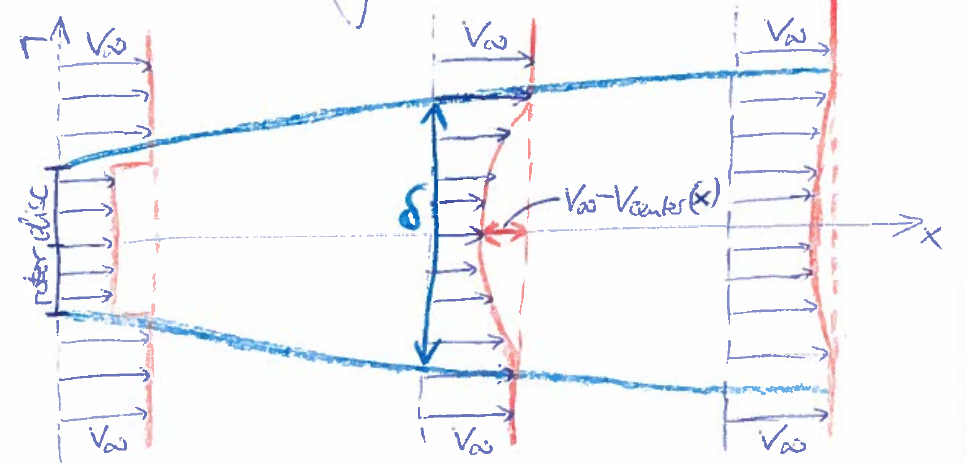
\includegraphics[width=.7\textwidth]{week5/negative-jet}\\
}

\begin{equation}
v_x(x,r) = v_\infty-v_\mathrm{center}(x)g\left(\frac{r}{\delta(x)}\right)
\end{equation}
\end{framed}